%% USEFUL LINKS:
%% -------------
%%
%% - UiO LaTeX guides:          https://www.mn.uio.no/ifi/tjenester/it/hjelp/latex/
%% - Mathematics:               https://en.wikibooks.org/wiki/LaTeX/Mathematics
%% - Physics:                   https://ctan.uib.no/macros/latex/contrib/physics/physics.pdf
%% - Basics of Tikz:            https://en.wikibooks.org/wiki/LaTeX/PGF/Tikz
%% - All the colors!            https://en.wikibooks.org/wiki/LaTeX/Colors
%% - How to make tables:        https://en.wikibooks.org/wiki/LaTeX/Tables
%% - Code listing styles:       https://en.wikibooks.org/wiki/LaTeX/Source_Code_Listings
%% - \includegraphics           https://en.wikibooks.org/wiki/LaTeX/Importing_Graphics
%% - Learn more about figures:  https://en.wikibooks.org/wiki/LaTeX/Floats,_Figures_and_Captions
%% - Automagic bibliography:    https://en.wikibooks.org/wiki/LaTeX/Bibliography_Management  (this one is kinda difficult the first time)
%%
%%                              (This document is of class "revtex4-1", the REVTeX Guide explains how the class works)
%%   REVTeX Guide:              http://www.physics.csbsju.edu/370/papers/Journal_Style_Manuals/auguide4-1.pdf
%%
%% COMPILING THE .pdf FILE IN THE LINUX IN THE TERMINAL
%% ----------------------------------------------------
%%
%% [terminal]$ pdflatex report_example.tex
%%
%% Run the command twice, always.
%%
%% When using references, footnotes, etc. you should run the following chain of commands:
%%
%% [terminal]$ pdflatex report_example.tex
%% [terminal]$ bibtex report_example
%% [terminal]$ pdflatex report_example.tex
%% [terminal]$ pdflatex report_example.tex
%%
%% This series of commands can of course be gathered into a single-line command:
%% [terminal]$ pdflatex report_example.tex && bibtex report_example.aux && pdflatex report_example.tex && pdflatex report_example.tex
%%
%% ----------------------------------------------------


\documentclass[english,notitlepage,reprint,nofootinbib]{revtex4-2}  % defines the basic parameters of the document
% For preview: skriv i terminal: latexmk -pdf -pvc filnavn
% If you want a single-column, remove "reprint"

% Allows special characters (including æøå)
\usepackage[utf8]{inputenc}
% \usepackage[english]{babel}

%% Note that you may need to download some of these packages manually, it depends on your setup.
%% I recommend downloading TeXMaker, because it includes a large library of the most common packages.

\usepackage{physics,amssymb}  % mathematical symbols (physics imports amsmath)
\usepackage{amsmath}
\usepackage{graphicx}         % include graphics such as plots
\usepackage{xcolor}           % set colors
\usepackage{hyperref}         % automagic cross-referencing
\usepackage{listings}         % display code
\usepackage{subfigure}        % imports a lot of cool and useful figure commands
% \usepackage{float}
%\usepackage[section]{placeins}
\usepackage{algorithm}
\usepackage[noend]{algpseudocode}
\usepackage{subfigure}
\usepackage{tikz}
\usetikzlibrary{quantikz}
% defines the color of hyperref objects
% Blending two colors:  blue!80!black  =  80% blue and 20% black
\hypersetup{ % this is just my personal choice, feel free to change things
	colorlinks,
	linkcolor={red!50!black},
	citecolor={blue!50!black},
	urlcolor={blue!80!black}}


% ===========================================

%\addbibresource{refs.bib} % Entries are in the "refs.bib" file

\begin{document}
	
	\title{Solving the Schrödinger Equation Using the 2D Crank-Nicolson Method}  % self-explanatory
	\author{Eloi Martaillé Richard,
	\
	Christophe Kristian Blomsen,
	\
	Ola Mårem
	\&
	Jørgen Armann Glenndal
    }
	\date{\today}                             % self-explanatory
	\noaffiliation                            % ignore this, but keep it.
	
	%This is how we create an abstract section.
	\begin{abstract}
Github link: \href{https://github.com/christopheblomsen/fys4150_pro5}{https://github.com/christopheblomsen/fys4150\_pro5}
\end{abstract}
	\maketitle	
	
	
	% ===========================================
	\section{Introduction} \label{sec:introduction}
	% ===========================================

	Light as always been an intriguing phenomena in physics. It began during the ancient Greece
	period were Democritus argued that all things in the universe are composed of indivisible 
	sub-components, i.e, particles. At the beginning of the eleventh century Ibn al-Haytham 
	wrote a physics book describing light no longer as a particle but as a wave, using a 
	pinhole lens to reflect, refract rays of light. This started a heated debate about the 
	wave-particle duality of light. All physicist joined one of the two side and tried to 
	prove that light was either a wave or a particle. \\
	
	In 1801, Thomas Young develop the double-slit experiment from Huygens-Fresnel principle
	resulting in the discovery of wave interference of light. \url{https://books.google.no/books?id=7AZGAAAAMAAJ&pg=PA1&redir_esc=y#v=onepage&q&f=false}
	
	This experiment did not solve the debate but the wave property of light began to dominate 
	scientific thinking. We will need the introduction of Quantum Mechanics to show that 
	light can behave as a particle and as a wave with the Schrödinger'equation being derived 
	from the wave equation. \\
	
	In this report we use the 2D time-dependent Schrodinger's equation to simulate a particle's
	motion in different slit methods, namely no slit, one, two or three slits. Since the 
	equation is a PDE being similar to the heat equation we will apply the Crank-Nicolson method.
	This is a finite difference method in time originally used to solve the heat equation
	\url{https://ui.adsabs.harvard.edu/abs/1947PCPS...43...50C/abstract}. \\
	
	In section \ref{sec:theory} we will overview the theoretical aspect of our problem by introducing
	the Schrödinger equation with some light quantum mechanics notion. Then in section \ref{sec:methods}
	we will introduce the numerical solution applied with the Crank-Nicolson method and the simulation
	done. After that we will briefly introduce all results obtained from the simulation in section 
	\ref{sec:results}. Finally we will discuss those results in section \ref{sec:discussion} and
	in section  \ref{sec:conclusion} we provide a short summary. 
	
	
	% ===========================================
	\section{Theory} \label{sec:theory}
	% ===========================================
	
	
	
	
	% ===========================================
	\section{Methods}\label{sec:methods}
	% ===========================================
	The bare Schrödinger equation can be written as 

	\begin{equation}\label{eq:bare Schrodinger}
		i \frac{\partial u}{\partial t} = -\frac{\partial^2 u}{\partial x^2} - \frac{\partial^2 u}{\partial y^2} + v(x,y) u.
	\end{equation} 
	
	In order to solve equation \ref{eq:bare Schrodinger} numerically, we must discetize all the terms and approximate
	the derivatives. The discretization is done by introducing a grid of points in the
	$xy$ plane containing all the values of $x$ and $y$ we will use. The time is discretized by using points, with equal spacing, along the time axis.\\ \\
	The first order time derivative on the left hand side of equation \ref{eq:bare Schrodinger} is approximated using the forward Euler method given by
	\begin{equation}
		\frac{\partial u}{\partial t} \approx \frac{u^{n+1}-u^n}{\Delta t},
	\end{equation}

	where $u^n$, in our case, is the dimentionless wavefunction in two dimentions.
	The superscript denotes the time step of $u$ and $\Delta t$ is the length of the time
	step, i.e. the spacing between points on the time axis.	For the second order spatial derivatives
	on the right hand side of equation \ref{eq:bare Schrodinger}
	we use Taylor approximations of second order. In the $x$ direction,
	the double spatial derivative is then given by
	
	\begin{equation}\label{ex:double x}
		\frac{\partial^2 u_{i,j}}{\partial x^2} \approx \frac{u_{i+1,j}-2u_{i,j}+u_{i-1,j}}{h^2},
	\end{equation}
	where the subscript denotes the $x$ and $y$ spatial step and $h$ is the spatial step size.
	The equation for the $y$ direction is a matter of flipping the variables from
	$x \rightarrow y$ and $i \rightarrow j$.
	in equation \ref{ex:double x}. The approximations for the derivatives are used in
	the Crank-Nicolson approach, which, is given by
	
	\begin{equation}
		\frac{u^{n+1}-u^{n}}{\Delta t} = \frac{1}{2}    \left(     F^{n+1} + F^n     \right),
	\end{equation}

	where the $F^{n+1}$ and $F^n$ terms are the right hand side of equation \ref{eq:bare Schrodinger}
	evaluated at different time steps. The superscript denotes the time step of the given variable, and $\Delta t$ is the length of the time step,
	i.e. the spacing between points on the time axis.\\ \\

	We rewrite equation \ref{eq:bare Schrodinger} into 

	Rewriting the terms in equation \ref{eq:bare Schrodinger}
	according to the Crank-Nicolson approach we get 

	\begin{equation}
	\frac{u^n_{i,j}}{\Delta t} = \frac{i}{2}\left(  (\frac{\partial^2 u}{\partial x^2} + \frac{\partial^2 u}{\partial y^2} + v(x,y) u        \right)
	\end{equation}
	

	
	
	
	Writing out all the terms in equation \ref{eq:bare Schrodinger}
	according to the Crank-Nicolson approach, and keeping the terms at time step $n+1$ on the left hand side and terms 
	at time step $n$ on the right hand side we get 


	

	


	
	
	% ===========================================
	\section{Results}\label{sec:results}
	% ===========================================

	\begin{figure}[h!]
		\centering
		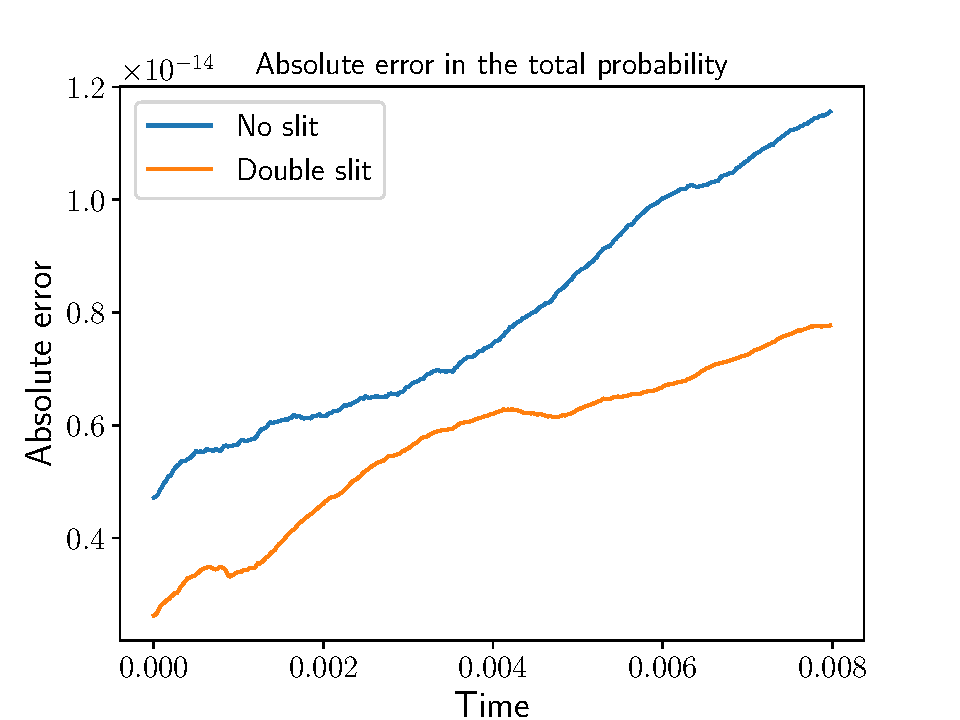
\includegraphics[scale=0.55]{figures/problem7_error.pdf}
		\caption{}
		\label{fig:prob7_error}
	\end{figure}

	\begin{figure}[h!]
		\centering
		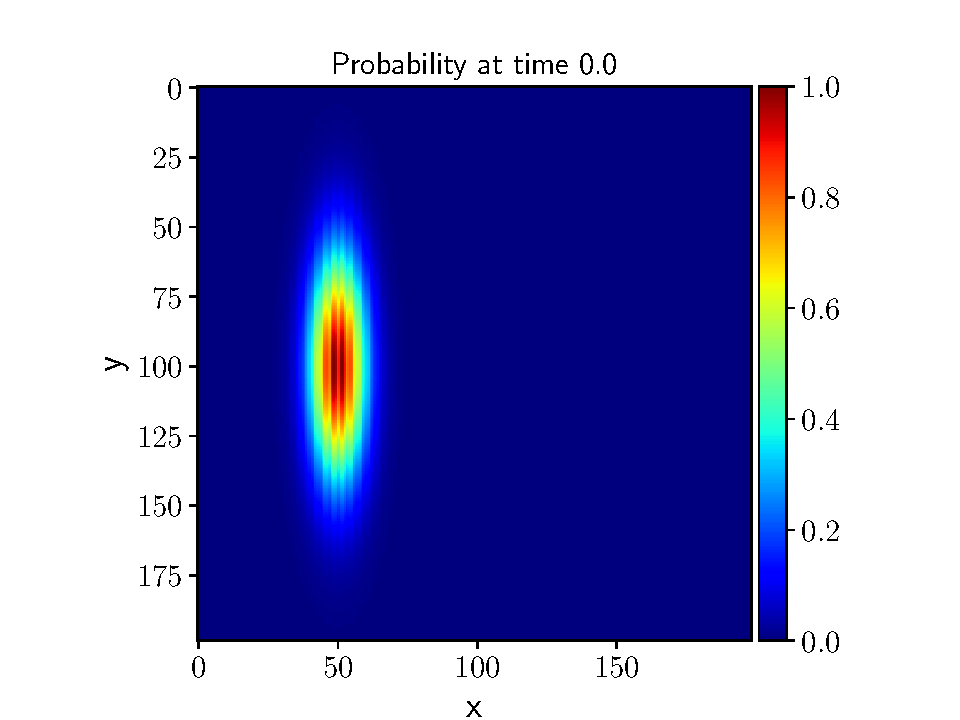
\includegraphics[scale=0.55]{figures/prob_plot_0.0.pdf}
		\caption{}
		\label{fig:prob_P0}
	\end{figure}

	\begin{figure}[h!]
		\centering
		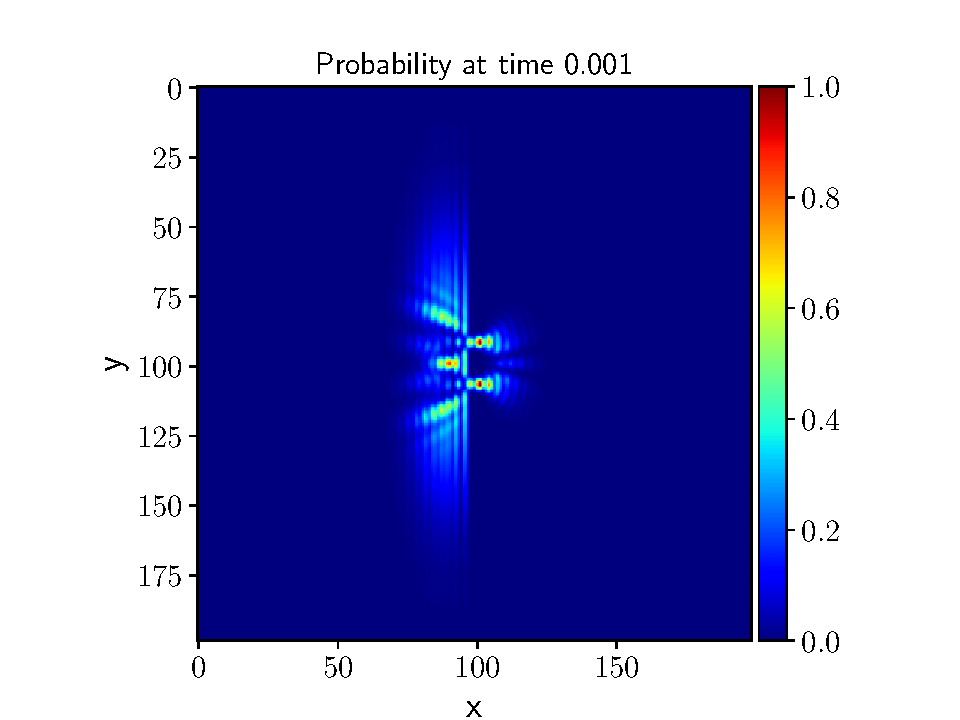
\includegraphics[scale=0.55]{figures/prob_plot_0.001.pdf}
		\caption{}
		\label{fig:prob8_P1}
	\end{figure}

	\begin{figure}[h!]
		\centering
		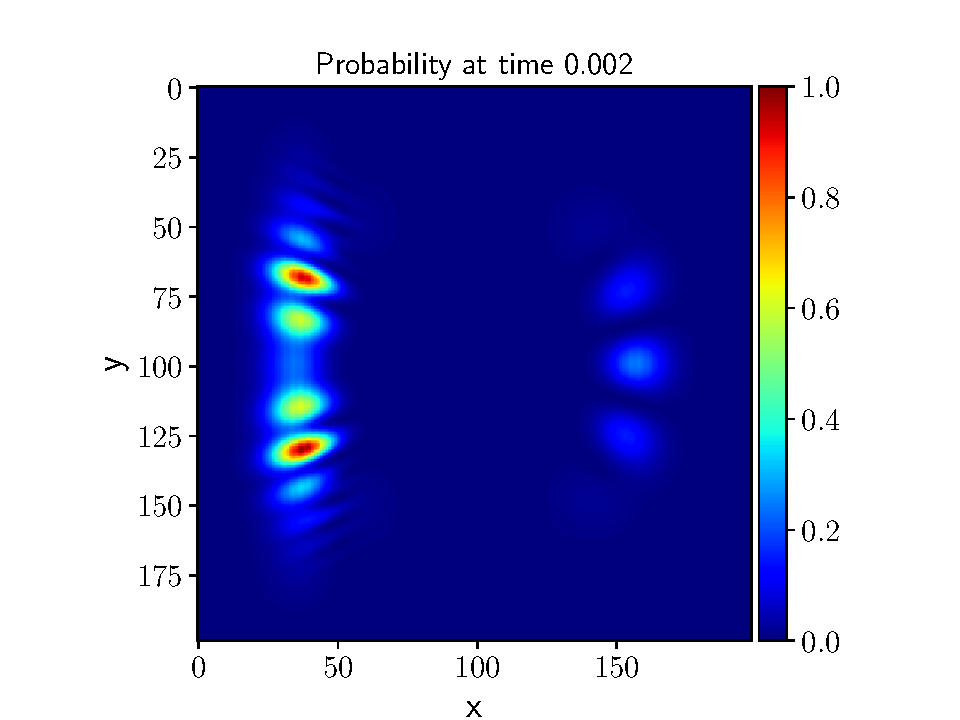
\includegraphics[scale=0.55]{figures/prob_plot_0.002.pdf}
		\caption{}
		\label{fig:prob8_P2}
	\end{figure}

	\begin{figure}[h!]
		\centering
		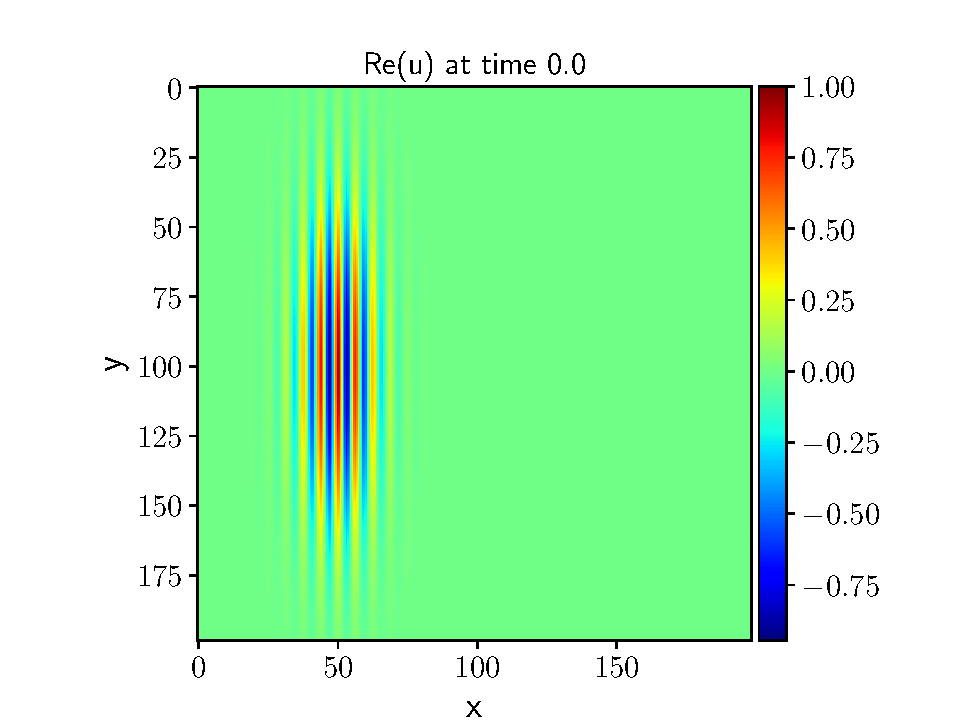
\includegraphics[scale=0.55]{figures/real_plot_0.0.pdf}
		\caption{}
		\label{fig:prob8_Re0}
	\end{figure}

	\begin{figure}[h!]
		\centering
		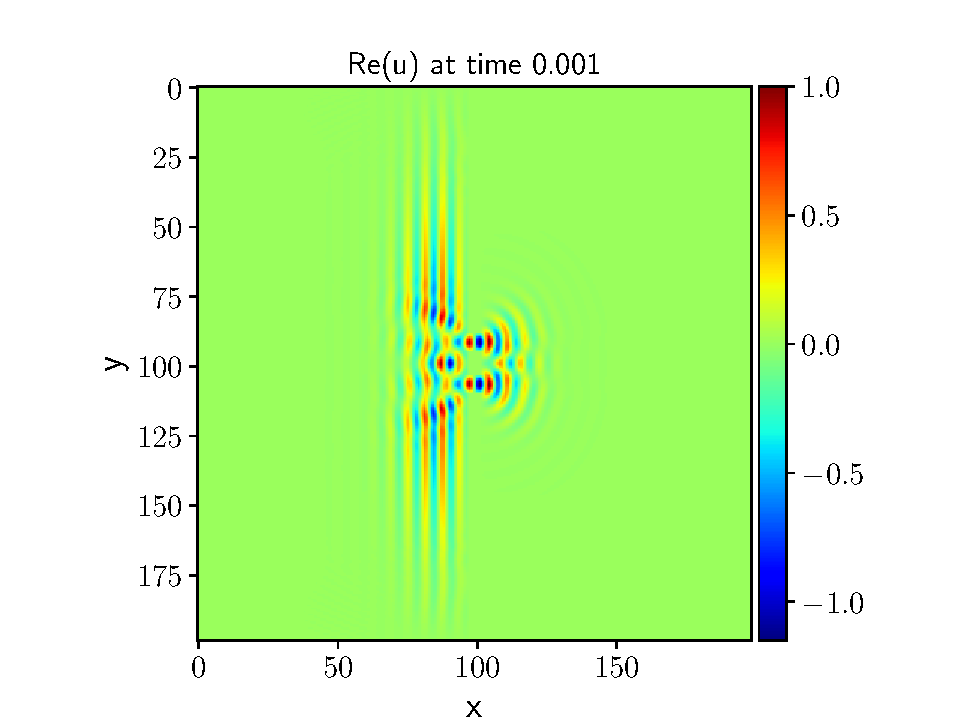
\includegraphics[scale=0.55]{figures/real_plot_0.001.pdf}
		\caption{}
		\label{fig:prob8_Re1}
	\end{figure}

	\begin{figure}[h!]
		\centering
		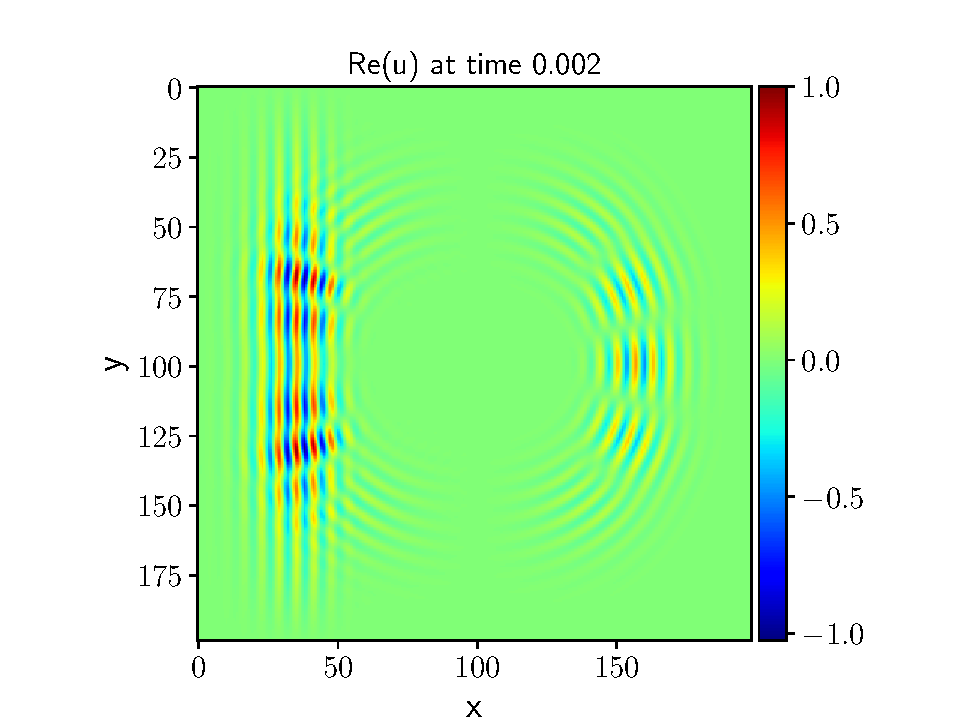
\includegraphics[scale=0.55]{figures/real_plot_0.002.pdf}
		\caption{}
		\label{fig:prob8_Re2}
	\end{figure}

	\begin{figure}[h!]
		\centering
		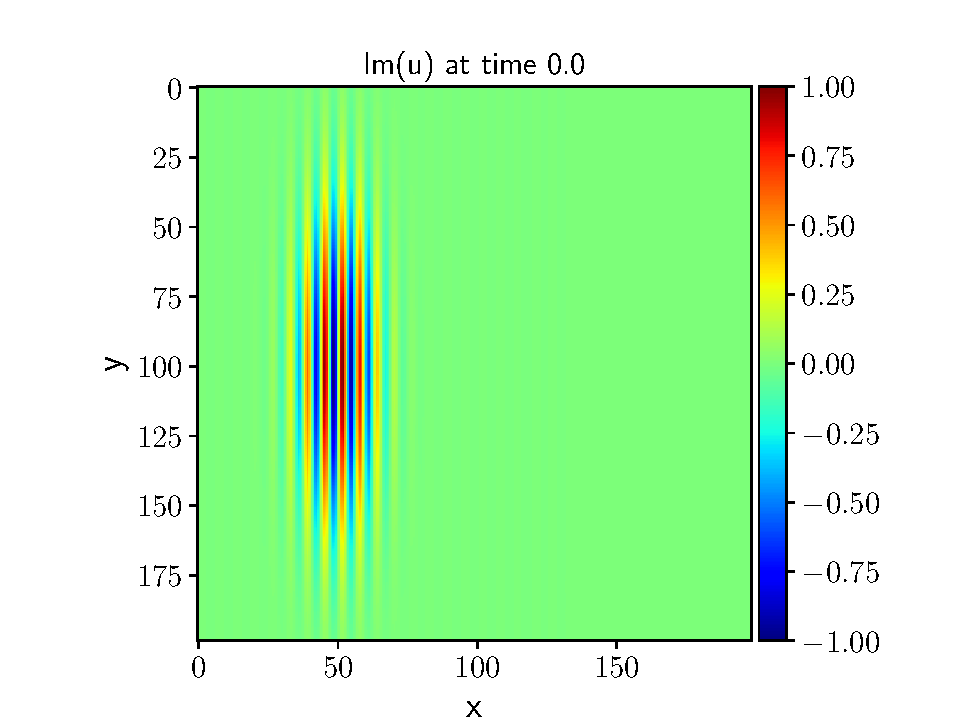
\includegraphics[scale=0.55]{figures/im_plot_0.0.pdf}
		\caption{}
		\label{fig:prob8_Im0}
	\end{figure}
	
	\begin{figure}[h!]
		\centering
		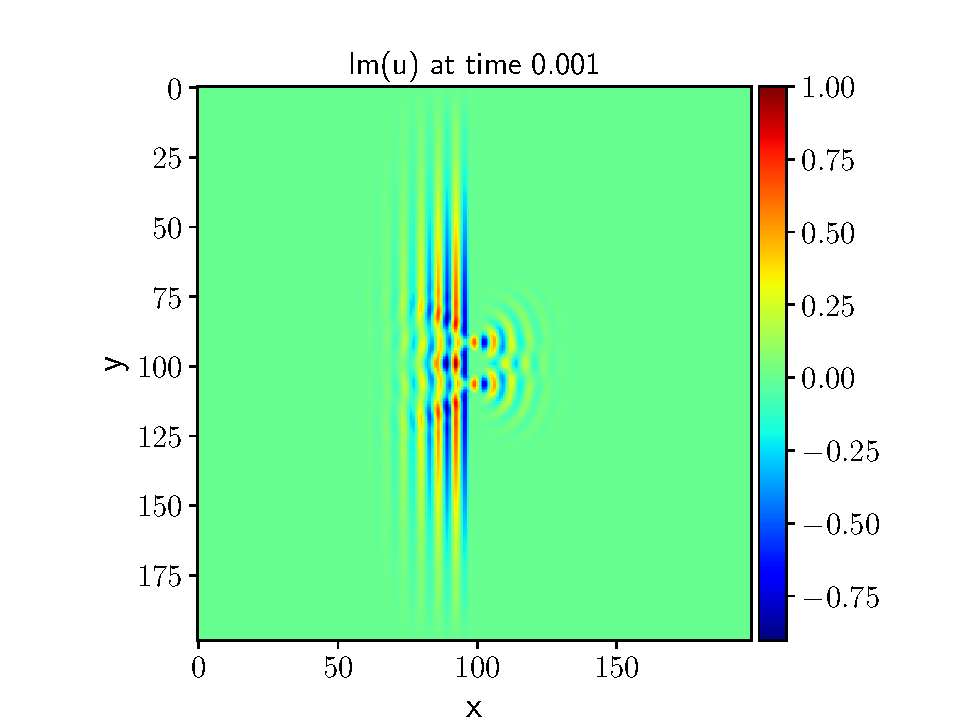
\includegraphics[scale=0.55]{figures/im_plot_0.001.pdf}
		\caption{}
		\label{fig:prob8_Im1}
	\end{figure}
	
	\begin{figure}[h!]
		\centering
		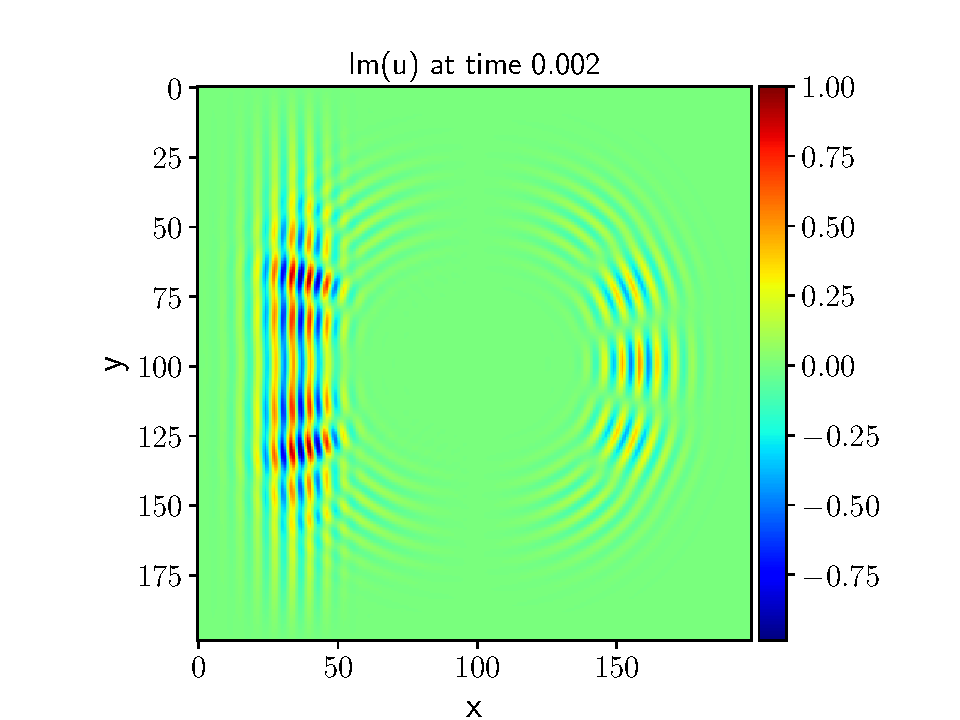
\includegraphics[scale=0.55]{figures/im_plot_0.002.pdf}
		\caption{}
		\label{fig:prob8_Im2}
	\end{figure}

	\begin{figure}[h!]
		\centering
		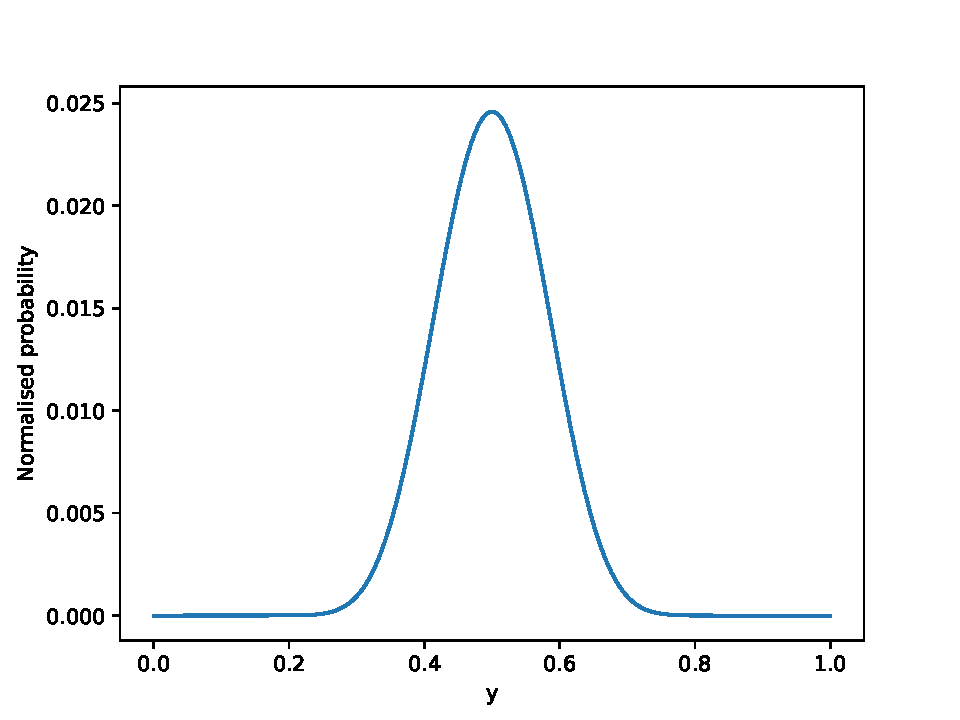
\includegraphics[scale=0.55]{figures/single_slit_detection.pdf}
		\caption{}
		\label{fig:prob9_single}
	\end{figure}
	
	\begin{figure}[h!]
		\centering
		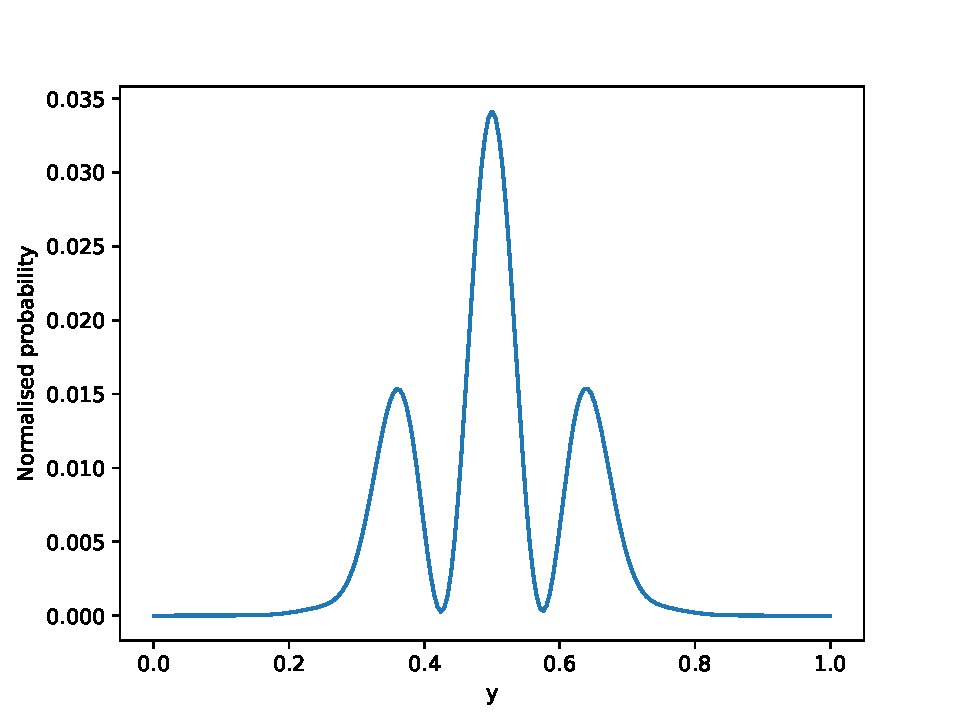
\includegraphics[scale=0.55]{figures/double_slit_detection.pdf}
		\caption{}
		\label{fig:prob9_double}
	\end{figure}
	
	\begin{figure}[h!]
		\centering
		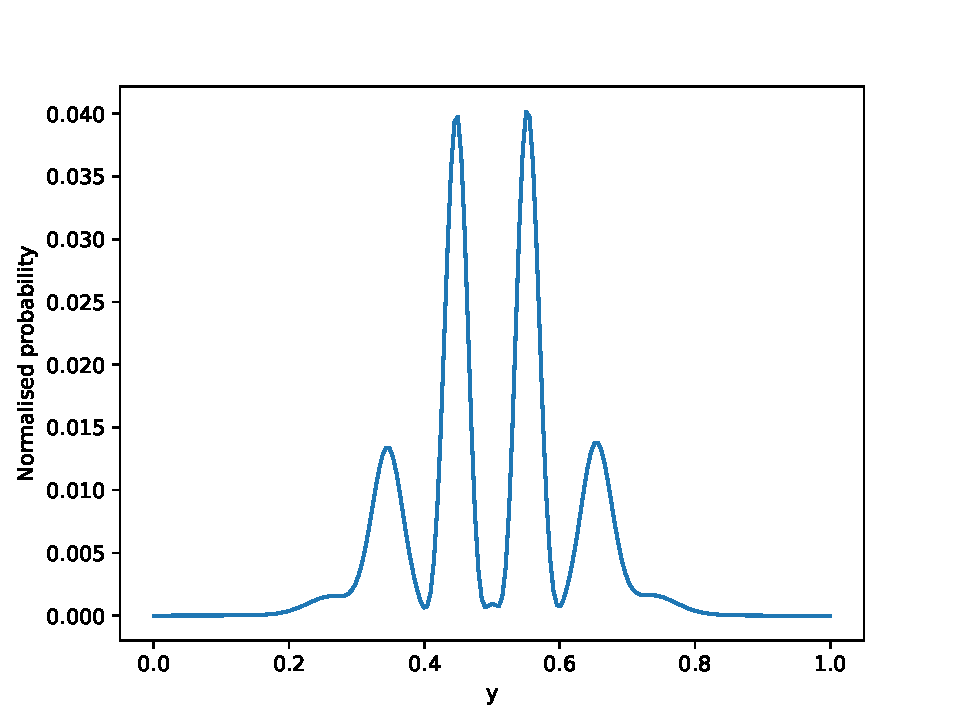
\includegraphics[scale=0.55]{figures/triple_slit_detection.pdf}
		\caption{}
		\label{fig:prob9_triple}
	\end{figure}
	% ===========================================
	\section{Discussion}\label{sec:discussion}
	% ===========================================
		heihei
	% ===========================================
	\section{Conclusion}\label{sec:conclusion}
	% ===========================================
	
	
	
	
	\onecolumngrid
	\section*{Refrences}
	%\bibliographystyle{apalike}
	\bibliography{refs}
	
	
\end{document}
